\documentclass{article}

\usepackage{graphicx}
\usepackage{listings}
\lstloadlanguages{Haskell}

\usepackage{amssymb}
\usepackage{amsmath}

\usepackage{tikz-cd}
\usetikzlibrary{cd}
\usepackage[utf8]{inputenc}

\usepackage{framed}
\usepackage{mdframed}

\newcommand{\id}[0]{\mathrm{id}}
\newcommand{\PostAdres}[0]{\mathtt{PostAdres}}
\newcommand{\Adres}[0]{\mathtt{Adres}}
\newcommand{\Huisnr}[0]{\mathtt{Huisnr}}

\newtheorem{definition}{Definitie}

\usepackage[dutch]{babel}

\begin{document}

\noindent Beste Jaap van Oosten. \\

Tijdens de bijeenkomst voor het Logic-seminar op dinsdag 4 april had ik het even met u over het concept ``\emph{lens}'' en of u die term misschien herkende uit de wereld van de categorie-theorie. Ik had toen beloofd dat ik u dit bericht zou sturen om dit concept beter uit te leggen. 

In de tussentijd heb ik wat verder gezocht en vond een hoop interessante literatuur uit zowel de informatica als de categorie-theory. Hoewel ik het nog niet volledig begrijp, vermoed ik dat dit een leuk onderwerk kan zijn voor mijn afstudeerproject.

In deze brief zal ik kort uitleggen wat \emph{lenses}, en in bredere vorm \emph{optics} zijn en wat ik er tot nu toe van begrijp. Ook zal kort beschrijven hoe ik ze tegen kom op mijn werk als developer en waarom ik dit onderwerp graag verder wil onderzoeken.

\section*{Wat is een \emph{lens}?}

The term \emph{lens} komt uit de wereld van de informatica en worden in het bijzonder gebruikt in de context van \emph{data-modelleren} en \emph{functioneel programmeren}. De simpelste vorm van een lens (een \emph{lawful-lens}) is als volgt te beschrijven:
\begin{definition}
	Laat $\mathcal{C}$ een categorie met eindige producten zijn. Een (lawful)-\emph{lens} van een `source'-object $S$ naar een `view'-object $V$ is een combinatie van twee pijlen $\mathtt{view}: S \to V$ en $\mathtt{set}: V \times S \to S$ zodanig dat de volgende diagrammen commutatief zijn:
    
    \[
	\begin{tikzcd}[]
		V \times S \arrow{r}[]{\mathtt{set}} \arrow{rd}[]{\pi_0} & S \arrow{d}{\mathtt{view}} \\
		& V
	\end{tikzcd} \hspace{40pt}
	\begin{tikzcd}[]
		S \arrow{r}[]{[\mathtt{view}, \id]} \arrow{rd}[]{\id} & V \times S \arrow{d}{\mathtt{set}} \\
		& S
	\end{tikzcd}
	\]
	\[
	\begin{tikzcd}[]
		V \times (V \times S) \arrow{r}[]{[\id, \mathtt{set}]} \arrow{d}{\pi_1} & V \times S \arrow{d}[]{\mathtt{set}} \\
		V \times S \arrow{r}[]{\mathtt{set}} & S
	\end{tikzcd}
	\]
\end{definition}


De intuïtie hierbij is dat je met een lens kunt \emph{focussen} op een specifieke waarde in een datastructuur. Vervolgens kun je deze waarde dan gemakkelijk wijzigen, zonder dat je de rest van de datastructuur aanpast.

\subsection*{Voorbeeld 1: \emph{Nederlandse postadressen}}

Neem als voorbeeld het de volgende datastructuur dat een Nederlands postadres modelleert:

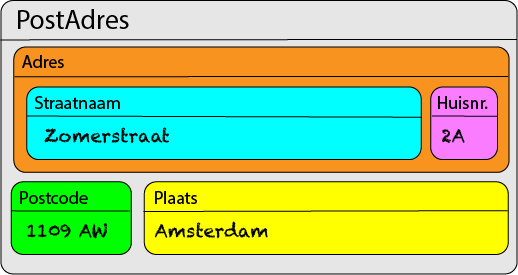
\includegraphics[width=0.5\linewidth]{datamodel-postadres.png}

In dit geval heb je bijvoorbeeld een lens van $\mathtt{PostAdres}$ naar $\mathtt{Plaats}$ waarbij $\mathtt{view}: \mathtt{PostAdres} \to \mathtt{Plaats}$ de plaatsnaam geeft en $\mathtt{set}: \mathtt{Plaats} \times \mathtt{PostAdres} \to \mathtt{Postadres}$ alleen plaatsnaam veranderd.

Je kunt ook denken aan complexe lens $g$ van $\mathtt{PostAdres}$ naar $\mathtt{Postcode}$ die rekening houd met de relatie tussen postcodes, straatnamen en plaatsnamen. In dit geval veranderd $\mathtt{set}_g: \mathtt{Postcode} \times \mathtt{PostAdres} \to \mathtt{PostAdres}$ niet alleen de postcode, maar ook de straat- en plaatsnaam in het adres.

\vspace{12pt}

\noindent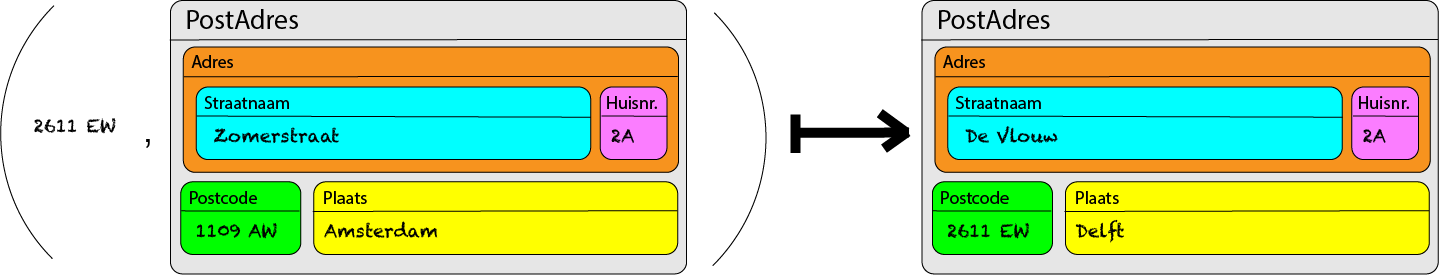
\includegraphics[width=\linewidth]{set-g.png}

\vspace{12pt}

De belangrijkste eigenschap van lenzen is je composities kunt maken. Denk bijvoorbeeld aan de lens van $\PostAdres$ naar $\Adres$ en de lens van $\Adres$ naar $\Huisnr$. Deze vormen samen een nieuwe lens van $\PostAdres$ naar $\Huisnr$. Dit begint dus al veel te lijken op een ``categorie van lenzen''.

\subsection*{Voorbeeld 2: \emph{Producten}}

Ik denk dat de lenzen op het product van twee objecten het meest simpele abstracte voorbeeld is. Laat $C,D \in \mathcal{C}_0$ en $S = C \times D$, dan zijn er twee lenzen $\sigma_0$, $\sigma_1$ met:

\begin{align*}
	\mathtt{view} [{\sigma_0}] &= \pi_0 &&: (C \times D) \to C \\
	\mathtt{set}  [{\sigma_0}] &= \id \times \pi_1 &&: C \times (C \times D) \to (C \times D) \\
	\\
	\mathtt{view} [{\sigma_1}] &= \pi_1 &&: (C \times D) \to D \\
	\mathtt{set}  [{\sigma_1}] &= \mathrm{rev} \circ \id \times \pi_0 &&: D \times (C \times D) \to (C \times D) \\
\end{align*}

Ik vermoed dat elke lens een compositie is van lenzen in deze vorm in een categorie met ``genoeg producten'', al weet ik dat niet zeker. 

\bigskip

Voor mijn werk werk ik vooral in de programmeertalen \emph{Haskell}, \emph{Idris} en \emph{PureScript}. Dit zogenaamde ``functionele programmeertalen'' waarin veel concepten uit de categorie-theorie wordt gebruikt. Je zou deze talen kunnen kunnen zien als een ``cartesian-closed category of types'', waarbij de objecten ``types'' zijn en de pijlen ``functions''. 

De lenzen waar ik vooral mee werk zijn iets algemener. Ik ben vaak de term ``\emph{Lawless lenses}'' tegengekomen, al snap ik nog niet helemaal waarom ze zo heten. Je zou een dergelijke lens als volgt kunnen samenvatten:

\begin{definition}
	Laat $\mathcal{C}$ een categorie met eindige producten zijn en $S,T,A,B \in \mathcal{C}_0$. Een \emph{lens} van $(S, T)$ naar $(A,B)$ is een paar pijlen $\mathtt{view}: S \to A$ en $\mathtt{set}: B \times S \to T$.
\end{definition}

Het idee hierbij is dat $\mathtt{set}$ niet alleen de waarden, maar ook de ``type'' van een object kan aanpassen. De lens $\sigma_0$ uit voorbeeld 2 zouden dan als volgt gedefinieerd kunnen worden (met $S = C \times D$ en $T = C' \times D$):
\begin{align*}
	\mathtt{view} [{\sigma_0}] &= \pi_0 &&: (C \times D) \to C \\
	\mathtt{set}  [{\sigma_0}] &= \id \times \pi_1 &&: C' \times (C \times D) \to (C' \times D) \\
\end{align*}

% https://www.twanvl.nl/blog/haskell/overloading-functional-references

Daarnaast wordt een lens in de (\emph{Haskell}) praktijk nooit gedefinïeerd als een paar $(\mathtt{view}, \mathtt{get})$. Inplaats daarvan wordt een functie gebruikt die in de Haskell-wereld de \emph{Van Laarhoven}-representatie wordt genoemd. Hierbij is een lens van $(S,T)$ naar $(A,B)$ een verzameling van functies \[
	\left\{ (FB)^A \to (FT)^S| F: \mathcal{C} \to \mathcal{C} \text{ een endofunctor}\right\}.
\]
Deze representatie is vooral handig in de praktijk omdat de compositie van lenzen op een zeer efficiënte manier kan worden geïmplementeerd. Je kunt vervolgens een $(\mathtt{view},\mathtt{set})$-lens omschrijven naar de \emph{Van Laarhoven}-representatie door \[
	\mathtt{lens}(g) = F(\mathtt{set}) \circ [g \circ \mathtt{view}, \id].
\]

\medskip

Algemener nog (vooral in \emph{Idris} en \emph{PureScript}, maar ook in \emph{Haskell}) gebruikt men de zogenaamde \emph{Profunctor}-representatie. Hierbij wordt een lens gezien als een pijl in een soort afgeleide categorie van Profunctors. Hoewel ik tot nu toe deze representatie het minst snap, boeit het mij het meeste.

Naast \emph{lenzen} bestaan er namelijk een hoop andere zogenaamde ``\emph{optics}''. Enkele voorbeelden zijn: \emph{Prism} (een co-\emph{lens}), \emph{Traversal}, \emph{Iso}, \emph{Grate}, \emph{Glass}. Hoewel ik deze dagelijks gebruik, snap ik ze nog niet goed genoeg om ze kort uit te leggen.

Wel begrijp ik dat elk van deze ``\emph{optics}'' een \emph{Profunctor}-representatie heeft en dat de meeste zijn ontdekt met behulp van categorie-theorie. Ook vermoed ik dat de \emph{van Laarhoven}-representatie slechts een speciale vorm is van de \emph{Profunctor}-representatie.

Het lijkt mij al heel interessant om de theorie achter deze optics en \emph{Profunctor}-representaties goed te begrijpen.


\section*{Wat ik wil onderzoeken}

Als de ``wiskundige'' onder de rest van de developers op mijn werk bestaat mijn taak vooral uit structuren begrijpbaar maken voor informatici. Dit komt hoofdzakelijk neer op het verzinnen van namen voor ``special cases'' van wiskundige structuren. Deze namen maakt de communicatie tussen het dev-team, het management en de klant een stuk makkelijker.

Naar mate ik meer met ``optics'' ben gaan werken, kreeg ik het vermoeden dat vrijwel alle structuren die ik een naam geef overeen komen met een optic (Voornamelijk \emph{Lens}, \emph{Prism} en \emph{Traversal}). Het zou daarom handig zijn om een methode te hebben waarmee alle optics geïdentificeerd worden.

Het liefste vind ik dus een methode waarmee ik een uitspraak als de volgende kan bewijzen:


\begin{center}
	\emph{``Voor een toepassing $X$ kan elke \emph{optic} beschreven worden als een compositie van de \emph{optics} $a\ldots z$.''}	
\end{center}


\vspace{4em}


\noindent Ik hoop dat ik u hiermee een idee heb gegeven voor wat \emph{lenzen} zijn en waarom ik denk dat het interessant is om ze te bestuderen door een categorie-theoretische bril. Daarnaast hoor ik graag van u of u denkt dat dit een goed onderwerp kan zijn voor mijn afstudeerproject.

\bigskip
 

\noindent Met vriendelijke groet,

\vspace{4em}

\noindent Roel Hemerik

% https://ncatlab.org/nlab/show/lens+%28in+computer+science%29

\end{document}

